\documentclass[xcolor=x11names,12pt]{beamer}
%\usetheme[secheader]{Boadilla} 
\mode<presentation>{\usetheme{I6pd2}}

\usepackage{multicol} 
\usepackage[utf8]{inputenc}
\usepackage[english]{babel}
\usepackage{grffile}
\usepackage{listings}
\usepackage{multirow}
\usepackage{amsmath}
\usepackage{pifont}
\usepackage{slashbox}
\usepackage{marvosym}
\usepackage{pgf}
\usepackage{pgfcore}
\usepackage{pgfbaseimage}
\usepackage{pgfbaselayers}
\usepackage{pgfbasepatterns}
\usepackage{pgfbaseplot}
\usepackage{pgfbaseshapes}
\usepackage{pgfbasesnakes}
\usepackage{tikz} 

\tikzset{normal/.style={ 
% The shape: 
rectangle,minimum size=6mm,rounded corners=3mm, 
% The rest 
very thick,draw=black!50, 
top color=white,bottom color=black!20, 
font=\ttfamily}}
\tikzset{arduino/.style={ 
% The shape: 
rectangle, 
% The size: 
minimum size=6mm, 
% The border: 
very thick, 
draw=blue!50!black!50, % 50% red and 50% black, 
% and that mixed with 50% white 
% The filling: 
top color=white, % a shading that is white at the top... 
bottom color=blue!50!black!20, % and something else at the bottom 
% Font 
font=\itshape 
}}
\tikzset{enceinte/.style={ 
% The shape: 
rectangle, 
% The size: 
minimum size=6mm, 
% The border: 
very thick, 
draw=yellow!90!black!50, % 50% red and 50% black, 
% and that mixed with 50% white 
% The filling: 
top color=white, % a shading that is white at the top... 
bottom color=yellow!90!black!20, % and something else at the bottom 
% Font 
font=\itshape 
}}

\tikzset{ordi/.style={ 
% The shape: 
rectangle, 
% The size: 
minimum size=6mm, 
% The border: 
very thick, 
draw=green!90!black!50, % 50% red and 50% black, 
% and that mixed with 50% white 
% The filling: 
top color=white, % a shading that is white at the top... 
bottom color=green!90!black!20, % and something else at the bottom 
% Font 
font=\itshape 
}}

\usetikzlibrary{through,shapes,arrows,decorations.pathmorphing,backgrounds,positioning,fit} 

\newcommand{\argmin}{\mathop{\mathrm{min}}}
\usepackage[orientation=portrait,size=a0,scale=1.4]{beamerposter}


\newcommand{\conf}[1]{\newcommand{\insertconf}{#1}}
\newenvironment{WholeWidthBox}[1]{
  \begin{columns}
    \begin{column}{0.98\textwidth}
      \begin{block}{#1}
        \begin{hfill}
}{
        \end{hfill}
      \end{block}
    \end{column}
  \end{columns}
}

\newcommand{\TwoBoxes}[7]{%Width1 Title1 Content1 Width2 Title2 Content2 MinHeight
  \begin{columns}
    \begin{column}{#1\textwidth}
      \begin{block}{#2}
        \begin{columns}
          \begin{column}{0.001\textwidth}
            \vspace{#7}
          \end{column}
          \begin{column}{\textwidth}
            \centering
            #3
          \end{column}
        \end{columns}       
      \end{block}
    \end{column}
    
    \begin{column}{#4\textwidth}
      \begin{block}{#5}
        \begin{columns}
          \begin{column}{0.001\textwidth}
            \vspace{#7}
          \end{column}
          \begin{column}{\textwidth}
            \centering
            #6
          \end{column}
        \end{columns}       
      \end{block}
    \end{column}
  \end{columns}
}


%Start of document



\tikzstyle{state}=[circle,
thick,
minimum size=1.0cm,
draw=blue!80,
fill=blue!20]
\tikzstyle{action}=[rectangle,thick,
minimum size=1.0cm,
draw=orange!80,
fill=orange!20]
\tikzstyle{element}=[rectangle,
line width=1.5mm,
minimum size=1.0cm,
draw=blue!80,
fill=blue!20]
\tikzstyle{action}=[rectangle,
line width=1.5mm,
minimum size=1.0cm,
draw=orange!80,
fill=orange!20]



\conf{European workshop on reinforcement learning}
\title{Inverse Reinforcement Learning through Structured Classification}
\author{\underline{Edouard Klein}$^{\dag\ddag}$, Matthieu Geist$^\dag$ and Olivier Pietquin$^{\dag\textrm{\Ankh}}$\\\texttt{firstname.lastname@supelec.fr}}
\date{\today}
\institute[Supélec]{$\dag$Equipe MaLIS (Supélec), France\\$\ddag$Equipe ABC UMR 7503 (LORIA-CNRS), France\\\Ankh UMI 2958 (GeorgiaTech - CNRS)}
\newlength{\columnheight}
\setlength{\columnheight}{105cm}


\begin{document}
\begin{frame}

%%%%%%%%%%%%% DEBUT PREMIERE LIGNE %%%%%%%%%%%%%%%%%
\begin{WholeWidthBox}{Introduction}
  Apprenticeship learning can be defined as learning control policies from demonstration by an expert. An efficient framework for it is inverse reinforcement learning
  (IRL). Based on the assumption that the expert maximizes a utility function, IRL aims at learning the underlying reward from example trajectories. Many IRL algorithms rely on the computation of \emph{feature expectations}, which is done through Monte Carlo simulation. In this paper, we introduce a temporal difference method, namely LSTD-$\mu$, to compute these feature expectations. This allows extending apprenticeship learning to a batch and off-policy setting.
\end{WholeWidthBox}

\vfill
%%%%%%%%%%%% DEBUT DEUXIEME LIGNE %%%%%%%%%%%%%%%%%%

\TwoBoxes{.48}{Setting}{
  \begin{columns}
    \begin{column}{.48\textwidth}
      
\includegraphics{Agent003.png}
    \end{column}
    \begin{column}{.48\textwidth}
      \begin{itemize}
      \item Expert's trace
      \item MDP : 
        \begin{itemize}
        \item State space $S$
        \item Action space $A$
        \item Unknown reward being maximized by the expert $R$
        \item Discount factor $\gamma$
        \item Transition probabilities $P$
        \end{itemize}
      \item Agent implementing a policy $\pi : S\rightarrow A$
      \end{itemize}
      
    \end{column}
  \end{columns}
}
{.48}{Assumptions and Goal}{
  \begin{itemize}
  \item Assumptions
    \begin{itemize}
    \item The expert is a RL agent
    \item One can access the expert's trace
    \item The agent has the same abilities as the expert
    \end{itemize}
  \item Goal : Infer the expert's reward
    \begin{itemize}
    \item apprenticeship of the expert's task
    \item Generalization of the policy over never-seen-before states
    \item Useful when rewards are hard to tune ({\it e.g.}, driving)
    \end{itemize}
  \end{itemize}
}
{15cm}
\vfill
%%%%%%%%%%%%%%%%%%%%%%%%%%%%%%%% TROISIEME LIGNE
\TwoBoxes{.38}{Feature Expectation}{
  \begin{equation*}
    V^\pi(s_t) = E\left[\left.\sum\limits_{i}\gamma^i r_{t+i}\right|\pi\right] = \theta^T\underbrace{E\left[\left.\sum\limits_{i}\gamma^i \phi(s_{t+i})\right|\pi\right]}_{\mu^\pi(s_t)}
  \end{equation*}
}{.58}{Importance of $\Delta \mu$}{
  \begin{equation*}
    \Delta V = |V^E(s_0) - V^\pi(s_0)| = |\theta^T\left(\mu_E(s_0) - \mu^\pi(s_0)\right)| \leq  ||\mu_E(s_0) - \mu^\pi(s_0)||_2 = \Delta\mu
  \end{equation*}
}
{6cm}
\vfill
%%%%%%%%%%%%%%%%%%%%%%%%%%%%% Quatrième ligne
  \begin{columns}
    \begin{column}{.48\textwidth}
    \begin{block}{LPSFBC}
      \begin{columns}
        \begin{column}{0.001\textwidth}
          \vspace{8cm}
        \end{column}
        \begin{column}{\textwidth}
          \centering
          Laius sur les classifieurs
        \end{column}
      \end{columns}       
      
    \end{block}
    \end{column}
    
    \begin{column}{.48\textwidth}
\begin{block}{Expert}
  \begin{columns}
    \begin{column}{0.001\textwidth}
      \vspace{8cm}
    \end{column}
    \begin{column}{\textwidth}
      \centering
      Parallèle sur l'expert
    \end{column}
  \end{columns}
\end{block}

    \end{column}
  \end{columns}
\vfill
%%%%%%%%%%%%%%%%%%%%%%Cinquième ligne

\begin{WholeWidthBox}{Putting it all together}
  \centering
  Blah blah blah
\end{WholeWidthBox}

%%%%%%%%%%%%%%%%%%%%%%Sixième ligne
  \begin{columns}
    \begin{column}{.48\textwidth}
      \begin{block}{Pseudo-code}
        \centering
        \fontsize{11pt}{11pt}\selectfont
        \resizebox{.55\columnwidth}{!}{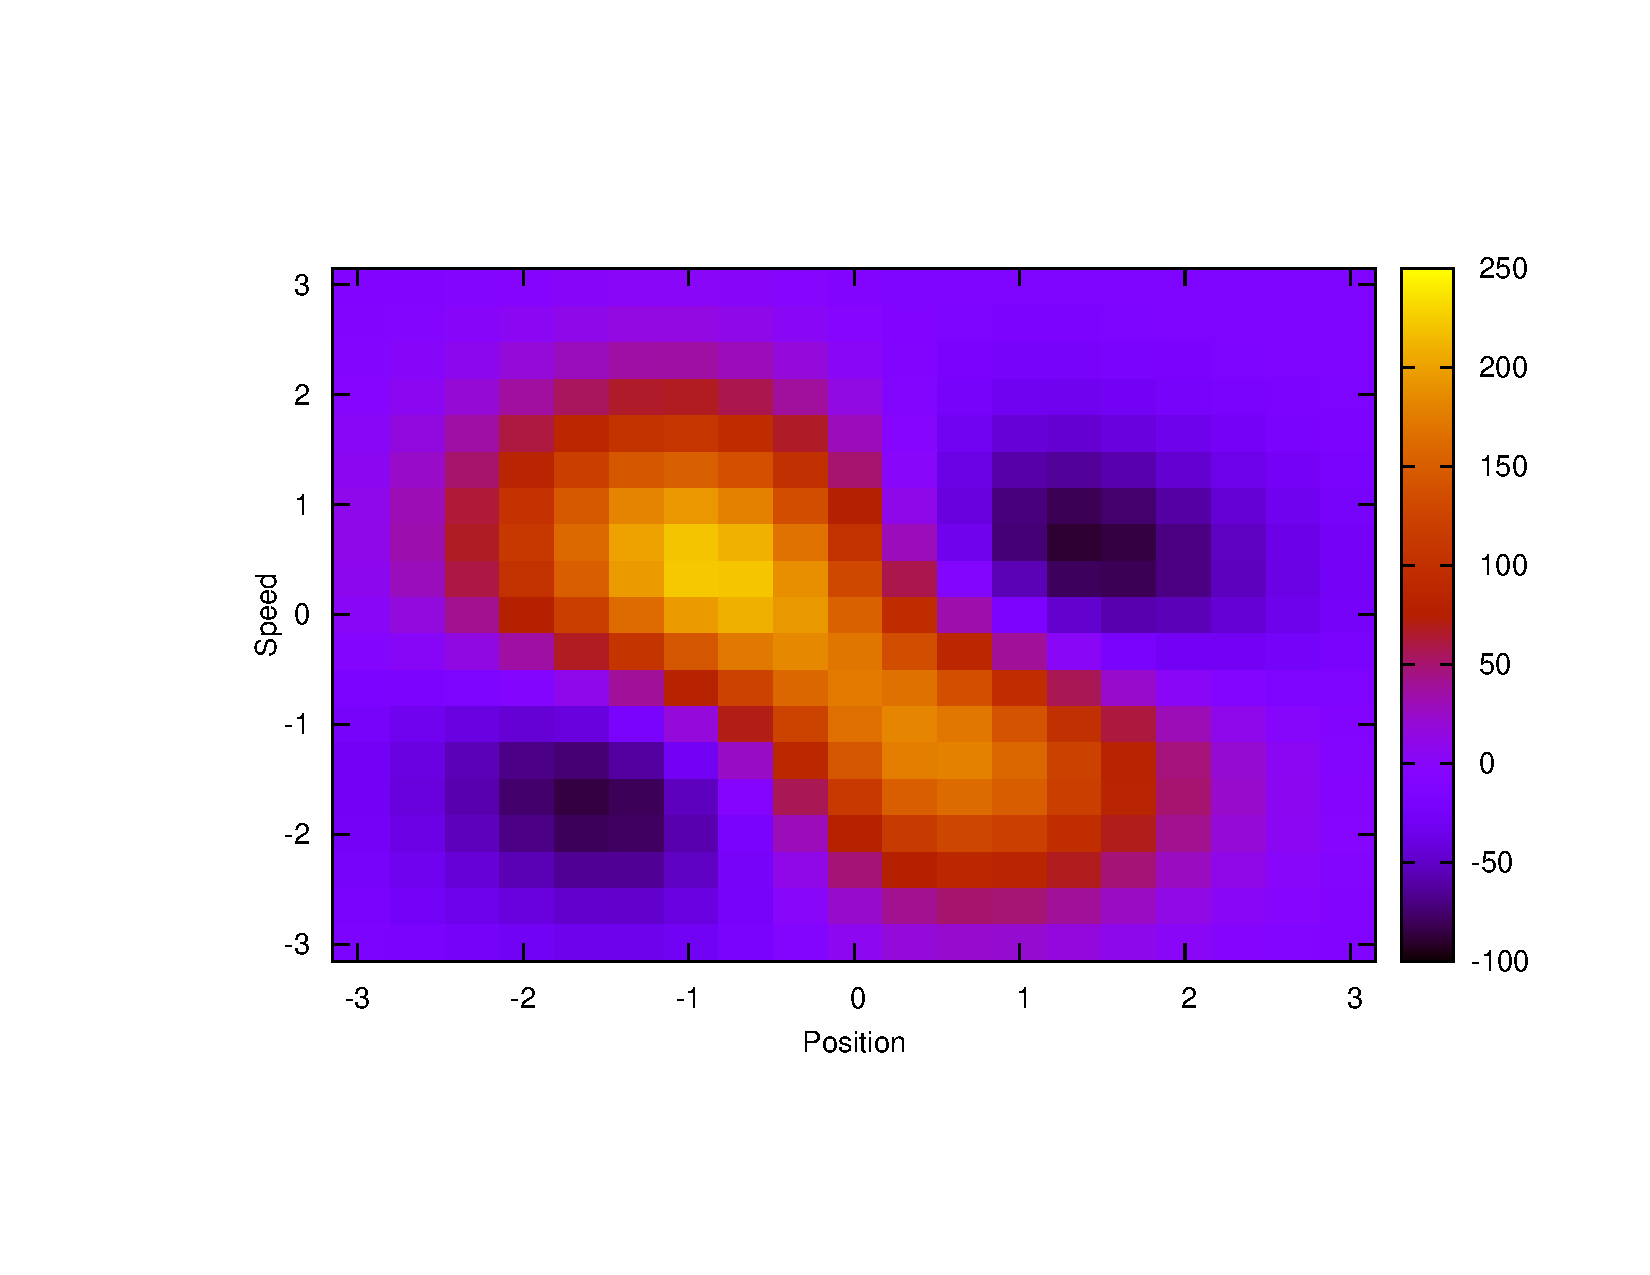
\includegraphics[width=\textwidth]{LAFEM_Exp3_Vagent.pdf}}
      \end{block}
    \end{column}
    \begin{column}{.48\textwidth}
      \begin{block}{Highway}
        \centering
        \fontsize{11pt}{11pt}\selectfont
        \resizebox{.55\columnwidth}{!}{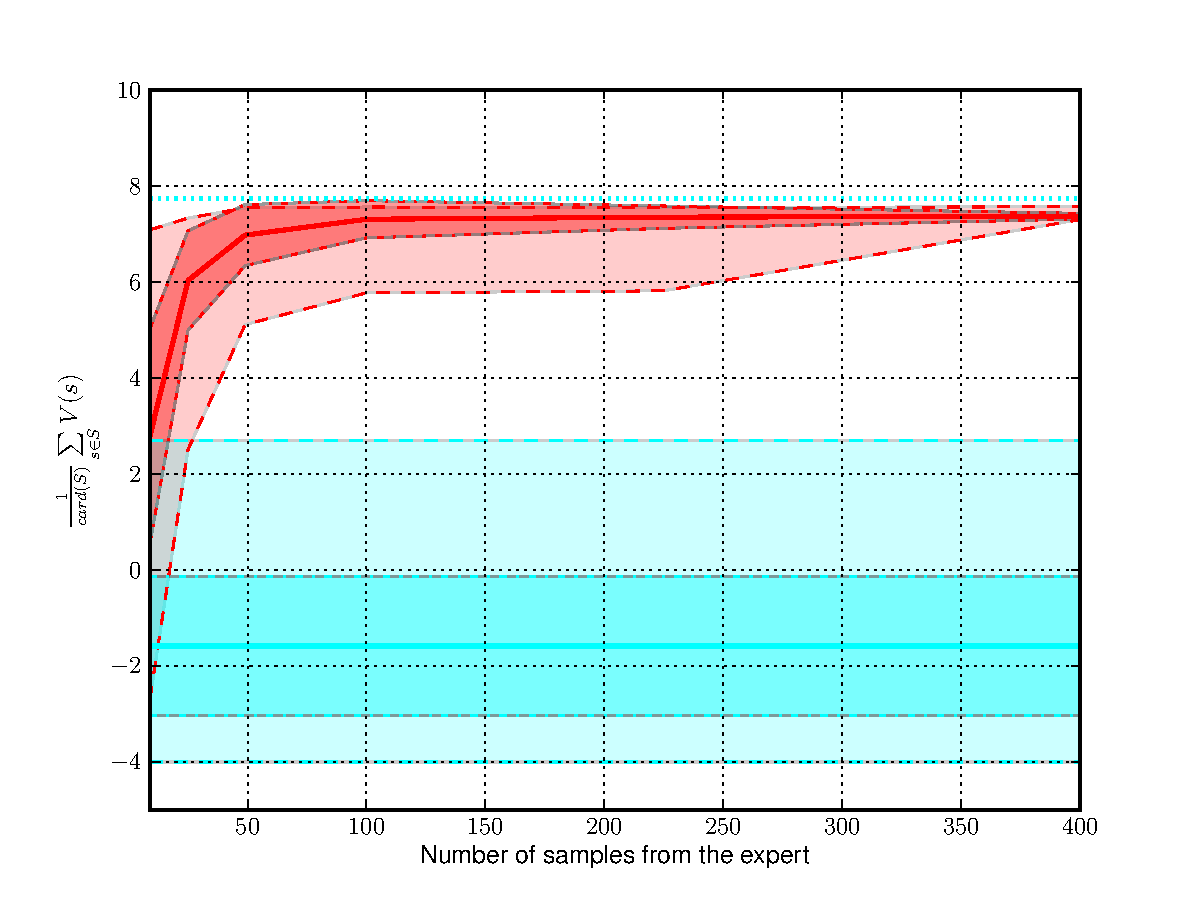
\includegraphics[width=\textwidth]{SCIRL_Exp3_fig1.pdf}}
      \end{block}
    \end{column}
  \end{columns}
  \begin{columns}
    \begin{column}{.48\textwidth}
      \begin{block}{GridWorld}
        \centering
        \fontsize{11pt}{11pt}\selectfont
        \resizebox{.55\columnwidth}{!}{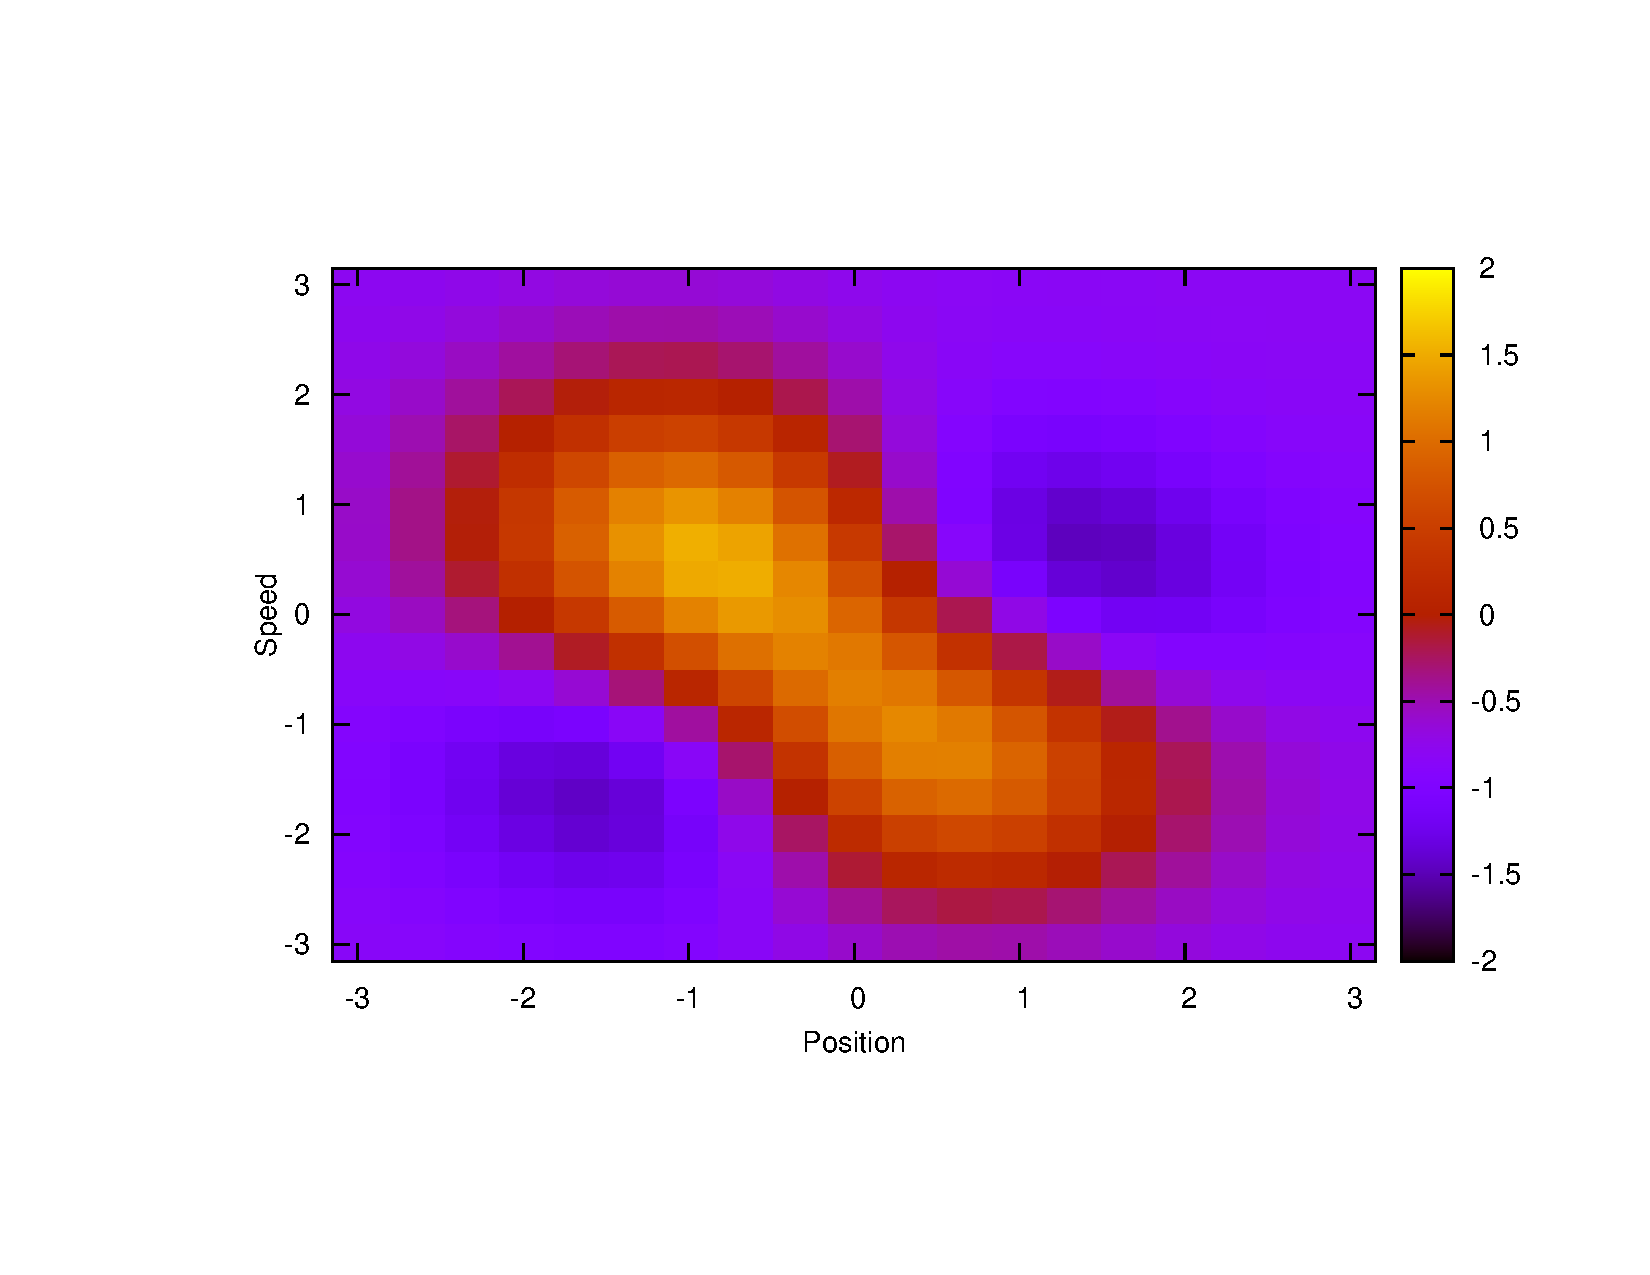
\includegraphics[width=\textwidth]{LAFEM_Exp3_Vexpert.pdf}}
      \end{block}
    \end{column}
    \begin{column}{.48\textwidth}
      \begin{block}{Inverted Pendulum}
        \centering
        \fontsize{11pt}{11pt}\selectfont
        \resizebox{.55\columnwidth}{!}{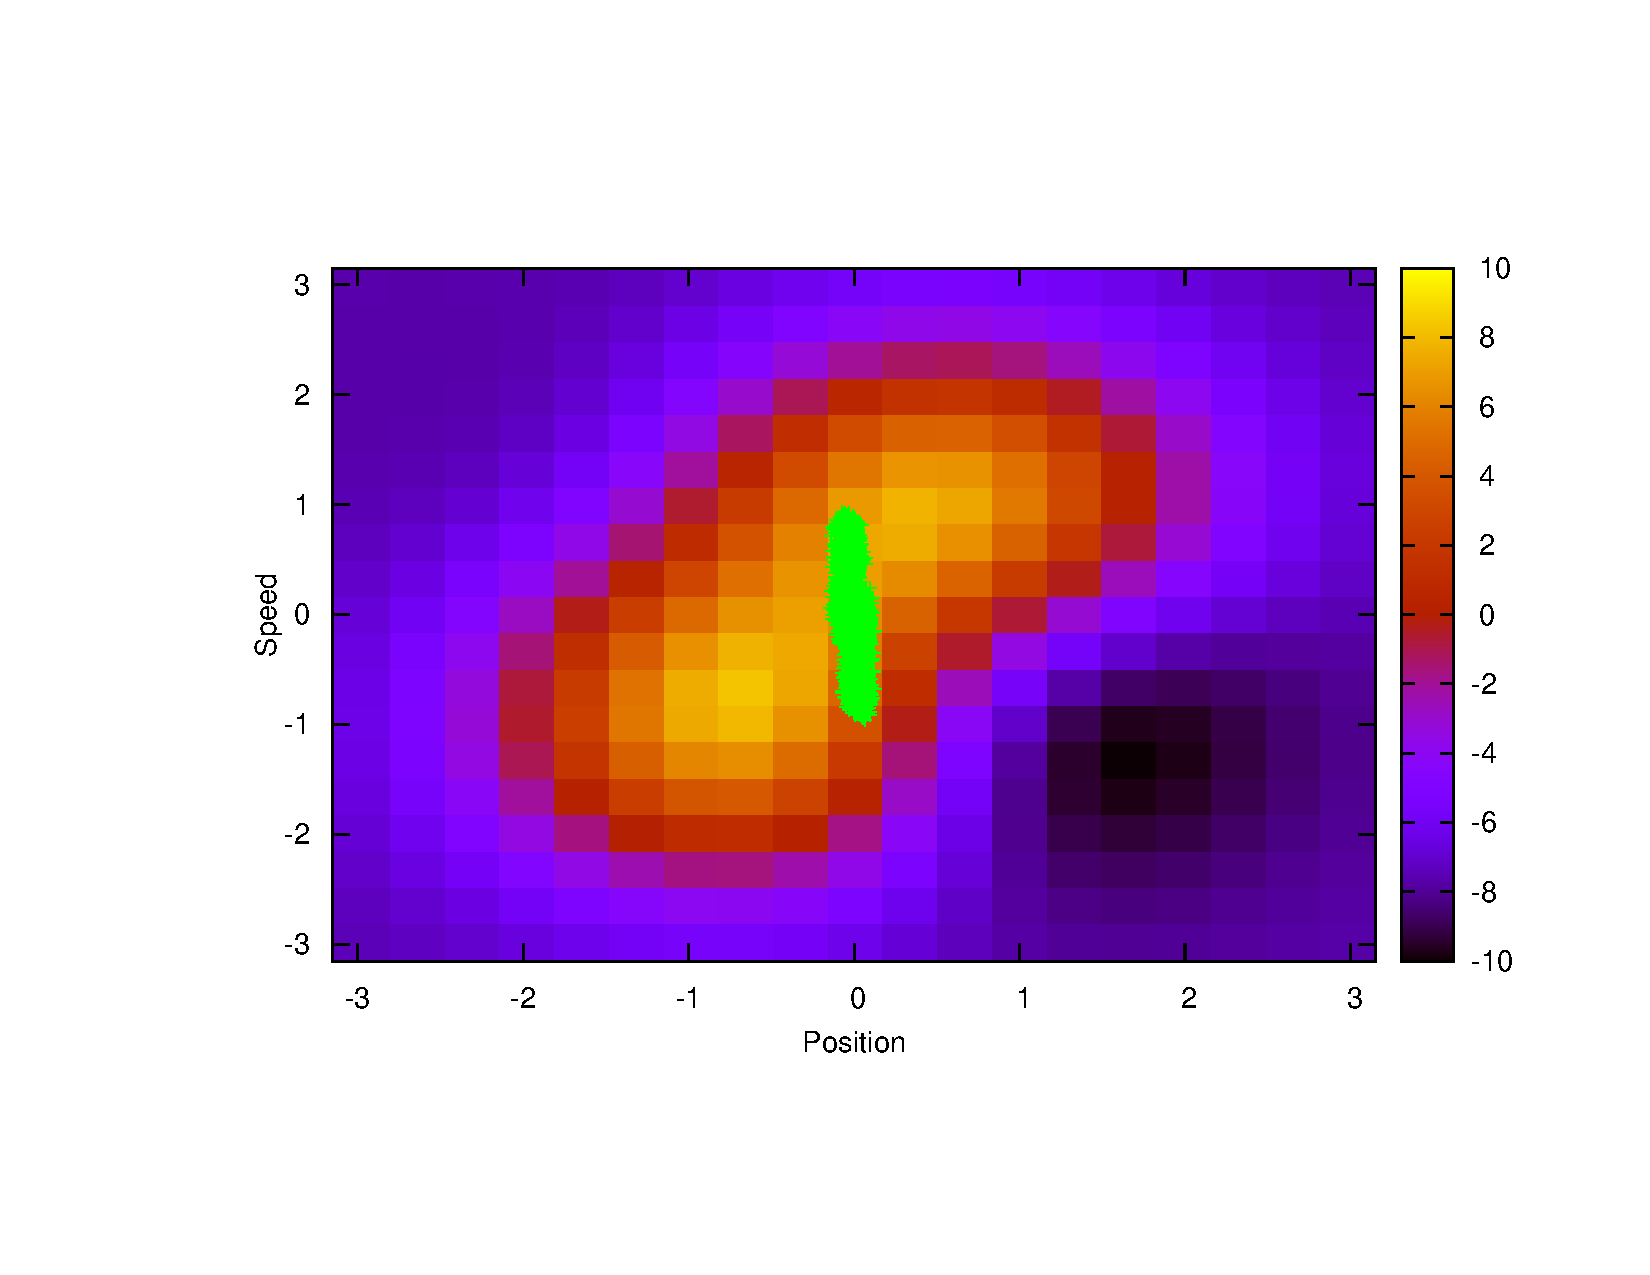
\includegraphics[width=\textwidth]{LAFEM_Exp3_lafem_R.pdf}}
      \end{block}
    \end{column}
  \end{columns}



\end{frame}
\end{document}
